% generated by Plantuml 1.2024.3       
\definecolor{plantucolor0000}{RGB}{0,0,0}
\definecolor{plantucolor0001}{RGB}{251,251,251}
\definecolor{plantucolor0002}{RGB}{119,119,119}
\definecolor{plantucolor0003}{RGB}{157,195,230}
\definecolor{plantucolor0004}{RGB}{85,85,85}
\definecolor{plantucolor0005}{RGB}{180,199,231}
\definecolor{plantucolor0006}{RGB}{217,179,217}
\definecolor{plantucolor0007}{RGB}{198,224,180}
\definecolor{plantucolor0008}{RGB}{174,214,241}
\definecolor{plantucolor0009}{RGB}{215,219,160}
\definecolor{plantucolor0010}{RGB}{255,217,102}
\definecolor{plantucolor0011}{RGB}{251,229,182}
\definecolor{plantucolor0012}{RGB}{24,24,24}
\definecolor{plantucolor0013}{RGB}{244,182,194}
\definecolor{plantucolor0014}{RGB}{68,68,68}
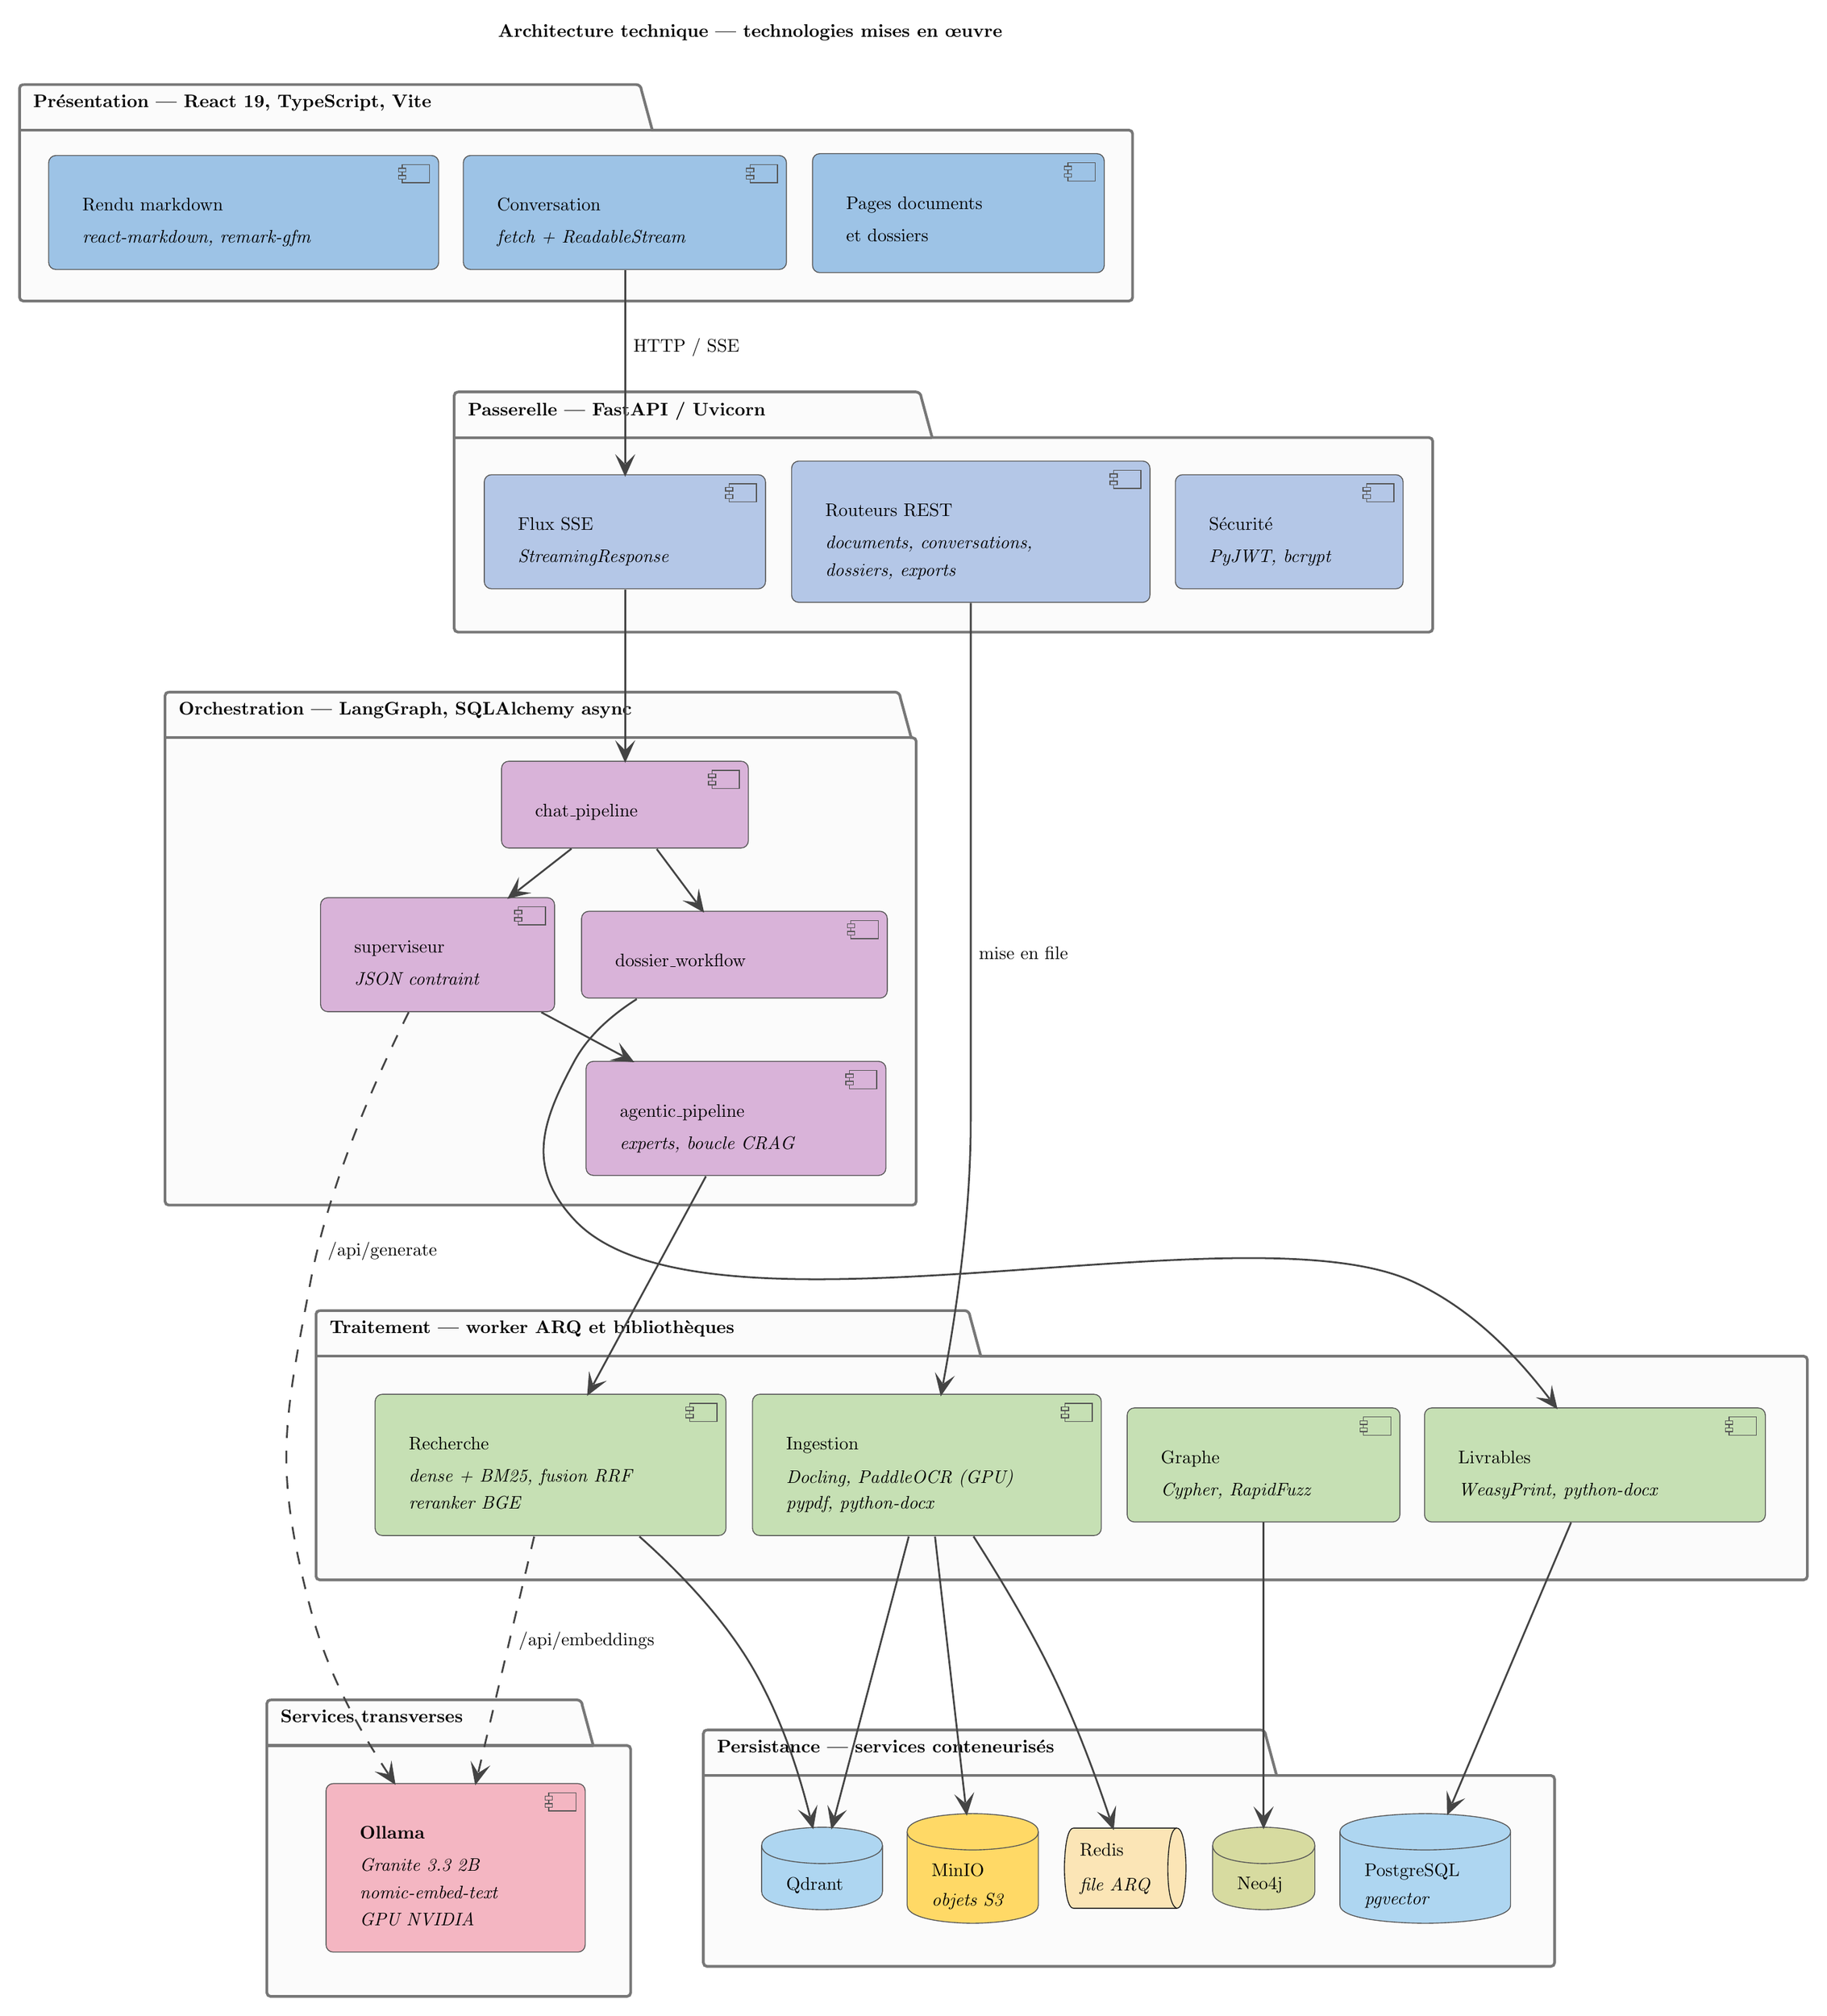
\begin{tikzpicture}[yscale=-1
,pstyle0/.style={color=plantucolor0002,fill=plantucolor0001,line width=1.5pt}
,pstyle1/.style={color=plantucolor0002,line width=1.5pt}
,pstyle2/.style={color=plantucolor0004,fill=plantucolor0003,line width=0.5pt}
,pstyle3/.style={color=plantucolor0004,fill=plantucolor0005,line width=0.5pt}
,pstyle4/.style={color=plantucolor0004,fill=plantucolor0006,line width=0.5pt}
,pstyle5/.style={color=plantucolor0004,fill=plantucolor0007,line width=0.5pt}
,pstyle6/.style={color=plantucolor0004,fill=plantucolor0008,line width=0.5pt}
,pstyle7/.style={color=plantucolor0004,line width=0.5pt}
,pstyle12/.style={color=plantucolor0004,fill=plantucolor0013,line width=0.5pt}
,pstyle13/.style={color=plantucolor0014,line width=1.0pt}
,pstyle14/.style={color=plantucolor0014,fill=plantucolor0014,line width=1.0pt}
,pstyle15/.style={color=plantucolor0014,line width=1.0pt,dash pattern=on 7.0pt off 7.0pt}
]
\node at (265.6072pt,10pt)[below right,color=black]{\textbf{Architecture technique — technologies mises en œuvre}};
\draw[pstyle0] (8pt,46.6699pt) -- (344.9174pt,46.6699pt) arc(270:360:3pt)  -- (353.9174pt,71.7378pt) -- (616pt,71.7378pt) arc(270:360:2pt)  -- (618pt,163.6699pt) arc(0:90:2pt)  -- (8pt,165.6699pt) arc(90:180:2pt)  -- (6pt,48.6699pt) arc(180:270:2pt) ;
\draw[pstyle1] (6pt,71.7378pt) -- (353.9174pt,71.7378pt);
\node at (10pt,48.6699pt)[below right,color=black]{\textbf{Présentation — React 19, TypeScript, Vite}};
\draw[pstyle0] (247pt,215.6699pt) -- (498.7825pt,215.6699pt) arc(270:360:3pt)  -- (507.7825pt,240.7378pt) -- (781pt,240.7378pt) arc(270:360:2pt)  -- (783pt,345.6699pt) arc(0:90:2pt)  -- (247pt,347.6699pt) arc(90:180:2pt)  -- (245pt,217.6699pt) arc(180:270:2pt) ;
\draw[pstyle1] (245pt,240.7378pt) -- (507.7825pt,240.7378pt);
\node at (249pt,217.6699pt)[below right,color=black]{\textbf{Passerelle — FastAPI / Uvicorn}};
\draw[pstyle0] (88pt,380.6699pt) -- (487.2706pt,380.6699pt) arc(270:360:3pt)  -- (496.2706pt,405.7378pt) -- (497pt,405.7378pt) arc(270:360:2pt)  -- (499pt,660.6699pt) arc(0:90:2pt)  -- (88pt,662.6699pt) arc(90:180:2pt)  -- (86pt,382.6699pt) arc(180:270:2pt) ;
\draw[pstyle1] (86pt,405.7378pt) -- (496.2706pt,405.7378pt);
\node at (90pt,382.6699pt)[below right,color=black]{\textbf{Orchestration — LangGraph, SQLAlchemy async}};
\draw[pstyle0] (171pt,720.6699pt) -- (525.5419pt,720.6699pt) arc(270:360:3pt)  -- (534.5419pt,745.7378pt) -- (987pt,745.7378pt) arc(270:360:2pt)  -- (989pt,866.6699pt) arc(0:90:2pt)  -- (171pt,868.6699pt) arc(90:180:2pt)  -- (169pt,722.6699pt) arc(180:270:2pt) ;
\draw[pstyle1] (169pt,745.7378pt) -- (534.5419pt,745.7378pt);
\node at (173pt,722.6699pt)[below right,color=black]{\textbf{Traitement — worker ARQ et bibliothèques}};
\draw[pstyle0] (384pt,951.1699pt) -- (688.1856pt,951.1699pt) arc(270:360:3pt)  -- (697.1856pt,976.2378pt) -- (848pt,976.2378pt) arc(270:360:2pt)  -- (850pt,1079.1699pt) arc(0:90:2pt)  -- (384pt,1081.1699pt) arc(90:180:2pt)  -- (382pt,953.1699pt) arc(180:270:2pt) ;
\draw[pstyle1] (382pt,976.2378pt) -- (697.1856pt,976.2378pt);
\node at (386pt,953.1699pt)[below right,color=black]{\textbf{Persistance — services conteneurisés}};
\draw[pstyle0] (144pt,934.6699pt) -- (312.4111pt,934.6699pt) arc(270:360:3pt)  -- (321.4111pt,959.7378pt) -- (340pt,959.7378pt) arc(270:360:2pt)  -- (342pt,1095.6699pt) arc(0:90:2pt)  -- (144pt,1097.6699pt) arc(90:180:2pt)  -- (142pt,936.6699pt) arc(180:270:2pt) ;
\draw[pstyle1] (142pt,959.7378pt) -- (321.4111pt,959.7378pt);
\node at (146pt,936.6699pt)[below right,color=black]{\textbf{Services transverses}};
\draw[pstyle2] (442pt,88.6699pt) arc (180:270:4pt) -- (446pt,84.6699pt) -- (598.4075pt,84.6699pt) arc (270:360:4pt) -- (602.4075pt,88.6699pt) -- (602.4075pt,146.0819pt) arc (0:90:4pt) -- (598.4075pt,150.0819pt) -- (446pt,150.0819pt) arc (90:180:4pt) -- (442pt,146.0819pt) -- cycle;
\draw[pstyle2] (582.4075pt,89.6699pt) rectangle (597.4075pt,99.6699pt);
\draw[pstyle2] (580.4075pt,91.6699pt) rectangle (584.4075pt,93.6699pt);
\draw[pstyle2] (580.4075pt,95.6699pt) rectangle (584.4075pt,97.6699pt);
\node at (457pt,104.6699pt)[below right,color=black]{Pages documents};
\node at (457pt,122.3759pt)[below right,color=black]{et dossiers};
\draw[pstyle2] (250pt,89.6699pt) arc (180:270:4pt) -- (254pt,85.6699pt) -- (423.665pt,85.6699pt) arc (270:360:4pt) -- (427.665pt,89.6699pt) -- (427.665pt,144.3578pt) arc (0:90:4pt) -- (423.665pt,148.3578pt) -- (254pt,148.3578pt) arc (90:180:4pt) -- (250pt,144.3578pt) -- cycle;
\draw[pstyle2] (407.665pt,90.6699pt) rectangle (422.665pt,100.6699pt);
\draw[pstyle2] (405.665pt,92.6699pt) rectangle (409.665pt,94.6699pt);
\draw[pstyle2] (405.665pt,96.6699pt) rectangle (409.665pt,98.6699pt);
\node at (265pt,105.6699pt)[below right,color=black]{Conversation};
\node at (265pt,123.3759pt)[below right,color=black]{\textit{fetch + ReadableStream}};
\draw[pstyle2] (22pt,89.6699pt) arc (180:270:4pt) -- (26pt,85.6699pt) -- (232.451pt,85.6699pt) arc (270:360:4pt) -- (236.451pt,89.6699pt) -- (236.451pt,144.3578pt) arc (0:90:4pt) -- (232.451pt,148.3578pt) -- (26pt,148.3578pt) arc (90:180:4pt) -- (22pt,144.3578pt) -- cycle;
\draw[pstyle2] (216.451pt,90.6699pt) rectangle (231.451pt,100.6699pt);
\draw[pstyle2] (214.451pt,92.6699pt) rectangle (218.451pt,94.6699pt);
\draw[pstyle2] (214.451pt,96.6699pt) rectangle (218.451pt,98.6699pt);
\node at (37pt,105.6699pt)[below right,color=black]{Rendu markdown};
\node at (37pt,123.3759pt)[below right,color=black]{\textit{react-markdown, remark-gfm}};
\draw[pstyle3] (641.5pt,265.1699pt) arc (180:270:4pt) -- (645.5pt,261.1699pt) -- (762.7324pt,261.1699pt) arc (270:360:4pt) -- (766.7324pt,265.1699pt) -- (766.7324pt,319.8578pt) arc (0:90:4pt) -- (762.7324pt,323.8578pt) -- (645.5pt,323.8578pt) arc (90:180:4pt) -- (641.5pt,319.8578pt) -- cycle;
\draw[pstyle3] (746.7324pt,266.1699pt) rectangle (761.7324pt,276.1699pt);
\draw[pstyle3] (744.7324pt,268.1699pt) rectangle (748.7324pt,270.1699pt);
\draw[pstyle3] (744.7324pt,272.1699pt) rectangle (748.7324pt,274.1699pt);
\node at (656.5pt,281.1699pt)[below right,color=black]{Sécurité};
\node at (656.5pt,298.8759pt)[below right,color=black]{\textit{PyJWT, bcrypt}};
\draw[pstyle3] (430.5pt,257.6699pt) arc (180:270:4pt) -- (434.5pt,253.6699pt) -- (623.5388pt,253.6699pt) arc (270:360:4pt) -- (627.5388pt,257.6699pt) -- (627.5388pt,327.3397pt) arc (0:90:4pt) -- (623.5388pt,331.3397pt) -- (434.5pt,331.3397pt) arc (90:180:4pt) -- (430.5pt,327.3397pt) -- cycle;
\draw[pstyle3] (607.5388pt,258.6699pt) rectangle (622.5388pt,268.6699pt);
\draw[pstyle3] (605.5388pt,260.6699pt) rectangle (609.5388pt,262.6699pt);
\draw[pstyle3] (605.5388pt,264.6699pt) rectangle (609.5388pt,266.6699pt);
\node at (445.5pt,273.6699pt)[below right,color=black]{Routeurs REST};
\node at (445.5pt,291.3759pt)[below right,color=black]{\textit{documents, conversations,}};
\node at (445.5pt,306.3578pt)[below right,color=black]{\textit{dossiers, exports}};
\draw[pstyle3] (261.5pt,265.1699pt) arc (180:270:4pt) -- (265.5pt,261.1699pt) -- (412.1612pt,261.1699pt) arc (270:360:4pt) -- (416.1612pt,265.1699pt) -- (416.1612pt,319.8578pt) arc (0:90:4pt) -- (412.1612pt,323.8578pt) -- (265.5pt,323.8578pt) arc (90:180:4pt) -- (261.5pt,319.8578pt) -- cycle;
\draw[pstyle3] (396.1612pt,266.1699pt) rectangle (411.1612pt,276.1699pt);
\draw[pstyle3] (394.1612pt,268.1699pt) rectangle (398.1612pt,270.1699pt);
\draw[pstyle3] (394.1612pt,272.1699pt) rectangle (398.1612pt,274.1699pt);
\node at (276.5pt,281.1699pt)[below right,color=black]{Flux SSE};
\node at (276.5pt,298.8759pt)[below right,color=black]{\textit{StreamingResponse}};
\draw[pstyle4] (271pt,422.6699pt) arc (180:270:4pt) -- (275pt,418.6699pt) -- (402.7171pt,418.6699pt) arc (270:360:4pt) -- (406.7171pt,422.6699pt) -- (406.7171pt,462.3759pt) arc (0:90:4pt) -- (402.7171pt,466.3759pt) -- (275pt,466.3759pt) arc (90:180:4pt) -- (271pt,462.3759pt) -- cycle;
\draw[pstyle4] (386.7171pt,423.6699pt) rectangle (401.7171pt,433.6699pt);
\draw[pstyle4] (384.7171pt,425.6699pt) rectangle (388.7171pt,427.6699pt);
\draw[pstyle4] (384.7171pt,429.6699pt) rectangle (388.7171pt,431.6699pt);
\node at (286pt,438.6699pt)[below right,color=black]{chat\_pipeline};
\draw[pstyle4] (171.5pt,497.6699pt) arc (180:270:4pt) -- (175.5pt,493.6699pt) -- (296.1737pt,493.6699pt) arc (270:360:4pt) -- (300.1737pt,497.6699pt) -- (300.1737pt,552.3578pt) arc (0:90:4pt) -- (296.1737pt,556.3578pt) -- (175.5pt,556.3578pt) arc (90:180:4pt) -- (171.5pt,552.3578pt) -- cycle;
\draw[pstyle4] (280.1737pt,498.6699pt) rectangle (295.1737pt,508.6699pt);
\draw[pstyle4] (278.1737pt,500.6699pt) rectangle (282.1737pt,502.6699pt);
\draw[pstyle4] (278.1737pt,504.6699pt) rectangle (282.1737pt,506.6699pt);
\node at (186.5pt,513.6699pt)[below right,color=black]{superviseur};
\node at (186.5pt,531.3759pt)[below right,color=black]{\textit{JSON contraint}};
\draw[pstyle4] (317.5pt,587.6699pt) arc (180:270:4pt) -- (321.5pt,583.6699pt) -- (478.3486pt,583.6699pt) arc (270:360:4pt) -- (482.3486pt,587.6699pt) -- (482.3486pt,642.3578pt) arc (0:90:4pt) -- (478.3486pt,646.3578pt) -- (321.5pt,646.3578pt) arc (90:180:4pt) -- (317.5pt,642.3578pt) -- cycle;
\draw[pstyle4] (462.3486pt,588.6699pt) rectangle (477.3486pt,598.6699pt);
\draw[pstyle4] (460.3486pt,590.6699pt) rectangle (464.3486pt,592.6699pt);
\draw[pstyle4] (460.3486pt,594.6699pt) rectangle (464.3486pt,596.6699pt);
\node at (332.5pt,603.6699pt)[below right,color=black]{agentic\_pipeline};
\node at (332.5pt,621.3759pt)[below right,color=black]{\textit{experts, boucle CRAG}};
\draw[pstyle4] (315pt,505.1699pt) arc (180:270:4pt) -- (319pt,501.1699pt) -- (479.1143pt,501.1699pt) arc (270:360:4pt) -- (483.1143pt,505.1699pt) -- (483.1143pt,544.8759pt) arc (0:90:4pt) -- (479.1143pt,548.8759pt) -- (319pt,548.8759pt) arc (90:180:4pt) -- (315pt,544.8759pt) -- cycle;
\draw[pstyle4] (463.1143pt,506.1699pt) rectangle (478.1143pt,516.1699pt);
\draw[pstyle4] (461.1143pt,508.1699pt) rectangle (465.1143pt,510.1699pt);
\draw[pstyle4] (461.1143pt,512.1699pt) rectangle (465.1143pt,514.1699pt);
\node at (330pt,521.1699pt)[below right,color=black]{dossier\_workflow};
\draw[pstyle5] (409pt,770.6699pt) arc (180:270:4pt) -- (413pt,766.6699pt) -- (596.7805pt,766.6699pt) arc (270:360:4pt) -- (600.7805pt,770.6699pt) -- (600.7805pt,840.3397pt) arc (0:90:4pt) -- (596.7805pt,844.3397pt) -- (413pt,844.3397pt) arc (90:180:4pt) -- (409pt,840.3397pt) -- cycle;
\draw[pstyle5] (580.7805pt,771.6699pt) rectangle (595.7805pt,781.6699pt);
\draw[pstyle5] (578.7805pt,773.6699pt) rectangle (582.7805pt,775.6699pt);
\draw[pstyle5] (578.7805pt,777.6699pt) rectangle (582.7805pt,779.6699pt);
\node at (424pt,786.6699pt)[below right,color=black]{Ingestion};
\node at (424pt,804.3759pt)[below right,color=black]{\textit{Docling, PaddleOCR (GPU)}};
\node at (424pt,819.3578pt)[below right,color=black]{\textit{pypdf, python-docx}};
\draw[pstyle5] (201.5pt,770.6699pt) arc (180:270:4pt) -- (205.5pt,766.6699pt) -- (390.4231pt,766.6699pt) arc (270:360:4pt) -- (394.4231pt,770.6699pt) -- (394.4231pt,840.3397pt) arc (0:90:4pt) -- (390.4231pt,844.3397pt) -- (205.5pt,844.3397pt) arc (90:180:4pt) -- (201.5pt,840.3397pt) -- cycle;
\draw[pstyle5] (374.4231pt,771.6699pt) rectangle (389.4231pt,781.6699pt);
\draw[pstyle5] (372.4231pt,773.6699pt) rectangle (376.4231pt,775.6699pt);
\draw[pstyle5] (372.4231pt,777.6699pt) rectangle (376.4231pt,779.6699pt);
\node at (216.5pt,786.6699pt)[below right,color=black]{Recherche};
\node at (216.5pt,804.3759pt)[below right,color=black]{\textit{dense + BM25, fusion RRF}};
\node at (216.5pt,819.3578pt)[below right,color=black]{\textit{reranker BGE}};
\draw[pstyle5] (615pt,778.1699pt) arc (180:270:4pt) -- (619pt,774.1699pt) -- (760.9579pt,774.1699pt) arc (270:360:4pt) -- (764.9579pt,778.1699pt) -- (764.9579pt,832.8578pt) arc (0:90:4pt) -- (760.9579pt,836.8578pt) -- (619pt,836.8578pt) arc (90:180:4pt) -- (615pt,832.8578pt) -- cycle;
\draw[pstyle5] (744.9579pt,779.1699pt) rectangle (759.9579pt,789.1699pt);
\draw[pstyle5] (742.9579pt,781.1699pt) rectangle (746.9579pt,783.1699pt);
\draw[pstyle5] (742.9579pt,785.1699pt) rectangle (746.9579pt,787.1699pt);
\node at (630pt,794.1699pt)[below right,color=black]{Graphe};
\node at (630pt,811.8759pt)[below right,color=black]{\textit{Cypher, RapidFuzz}};
\draw[pstyle5] (778.5pt,778.1699pt) arc (180:270:4pt) -- (782.5pt,774.1699pt) -- (961.9125pt,774.1699pt) arc (270:360:4pt) -- (965.9125pt,778.1699pt) -- (965.9125pt,832.8578pt) arc (0:90:4pt) -- (961.9125pt,836.8578pt) -- (782.5pt,836.8578pt) arc (90:180:4pt) -- (778.5pt,832.8578pt) -- cycle;
\draw[pstyle5] (945.9125pt,779.1699pt) rectangle (960.9125pt,789.1699pt);
\draw[pstyle5] (943.9125pt,781.1699pt) rectangle (947.9125pt,783.1699pt);
\draw[pstyle5] (943.9125pt,785.1699pt) rectangle (947.9125pt,787.1699pt);
\node at (793.5pt,794.1699pt)[below right,color=black]{Livrables};
\node at (793.5pt,811.8759pt)[below right,color=black]{\textit{WeasyPrint, python-docx}};
\draw[pstyle6] (732pt,1007.1699pt) ..controls (732pt,997.1699pt) and (778.9pt,997.1699pt) .. (778.9pt,997.1699pt) ..controls (778.9pt,997.1699pt) and (825.8pt,997.1699pt) .. (825.8pt,1007.1699pt) -- (825.8pt,1047.4959pt) ..controls (825.8pt,1057.4959pt) and (778.9pt,1057.4959pt) .. (778.9pt,1057.4959pt) ..controls (778.9pt,1057.4959pt) and (732pt,1057.4959pt) .. (732pt,1047.4959pt) -- (732pt,1007.1699pt);
\draw[pstyle7] (732pt,1007.1699pt) ..controls (732pt,1017.1699pt) and (778.9pt,1017.1699pt) .. (778.9pt,1017.1699pt) ..controls (778.9pt,1017.1699pt) and (825.8pt,1017.1699pt) .. (825.8pt,1007.1699pt);
\node at (742pt,1021.1699pt)[below right,color=black]{PostgreSQL};
\node at (742pt,1037.514pt)[below right,color=black]{\textit{pgvector}};
\draw[pstyle6] (414pt,1014.6699pt) ..controls (414pt,1004.6699pt) and (447.2341pt,1004.6699pt) .. (447.2341pt,1004.6699pt) ..controls (447.2341pt,1004.6699pt) and (480.4683pt,1004.6699pt) .. (480.4683pt,1014.6699pt) -- (480.4683pt,1040.014pt) ..controls (480.4683pt,1050.014pt) and (447.2341pt,1050.014pt) .. (447.2341pt,1050.014pt) ..controls (447.2341pt,1050.014pt) and (414pt,1050.014pt) .. (414pt,1040.014pt) -- (414pt,1014.6699pt);
\draw[pstyle7] (414pt,1014.6699pt) ..controls (414pt,1024.6699pt) and (447.2341pt,1024.6699pt) .. (447.2341pt,1024.6699pt) ..controls (447.2341pt,1024.6699pt) and (480.4683pt,1024.6699pt) .. (480.4683pt,1014.6699pt);
\node at (424pt,1028.6699pt)[below right,color=black]{Qdrant};
\draw[color=plantucolor0004,fill=plantucolor0009,line width=0.5pt] (662pt,1014.6699pt) ..controls (662pt,1004.6699pt) and (690.103pt,1004.6699pt) .. (690.103pt,1004.6699pt) ..controls (690.103pt,1004.6699pt) and (718.2061pt,1004.6699pt) .. (718.2061pt,1014.6699pt) -- (718.2061pt,1040.014pt) ..controls (718.2061pt,1050.014pt) and (690.103pt,1050.014pt) .. (690.103pt,1050.014pt) ..controls (690.103pt,1050.014pt) and (662pt,1050.014pt) .. (662pt,1040.014pt) -- (662pt,1014.6699pt);
\draw[pstyle7] (662pt,1014.6699pt) ..controls (662pt,1024.6699pt) and (690.103pt,1024.6699pt) .. (690.103pt,1024.6699pt) ..controls (690.103pt,1024.6699pt) and (718.2061pt,1024.6699pt) .. (718.2061pt,1014.6699pt);
\node at (672pt,1028.6699pt)[below right,color=black]{Neo4j};
\draw[color=plantucolor0004,fill=plantucolor0010,line width=0.5pt] (494pt,1007.1699pt) ..controls (494pt,997.1699pt) and (530.0818pt,997.1699pt) .. (530.0818pt,997.1699pt) ..controls (530.0818pt,997.1699pt) and (566.1636pt,997.1699pt) .. (566.1636pt,1007.1699pt) -- (566.1636pt,1047.4959pt) ..controls (566.1636pt,1057.4959pt) and (530.0818pt,1057.4959pt) .. (530.0818pt,1057.4959pt) ..controls (530.0818pt,1057.4959pt) and (494pt,1057.4959pt) .. (494pt,1047.4959pt) -- (494pt,1007.1699pt);
\draw[pstyle7] (494pt,1007.1699pt) ..controls (494pt,1017.1699pt) and (530.0818pt,1017.1699pt) .. (530.0818pt,1017.1699pt) ..controls (530.0818pt,1017.1699pt) and (566.1636pt,1017.1699pt) .. (566.1636pt,1007.1699pt);
\node at (504pt,1021.1699pt)[below right,color=black]{MinIO};
\node at (504pt,1037.514pt)[below right,color=black]{\textit{objets S3}};
\draw[color=plantucolor0012,fill=plantucolor0011,line width=0.5pt] (585.5pt,1005.1699pt) -- (642.3585pt,1005.1699pt) ..controls (647.3585pt,1005.1699pt) and (647.3585pt,1027.1948pt) .. (647.3585pt,1027.1948pt) ..controls (647.3585pt,1027.1948pt) and (647.3585pt,1049.2197pt) .. (642.3585pt,1049.2197pt) -- (585.5pt,1049.2197pt) ..controls (580.5pt,1049.2197pt) and (580.5pt,1027.1948pt) .. (580.5pt,1027.1948pt) ..controls (580.5pt,1027.1948pt) and (580.5pt,1005.1699pt) .. (585.5pt,1005.1699pt);
\draw[color=plantucolor0012,line width=0.5pt] (642.3585pt,1005.1699pt) ..controls (637.3585pt,1005.1699pt) and (637.3585pt,1027.1948pt) .. (637.3585pt,1027.1948pt) ..controls (637.3585pt,1049.2197pt) and (642.3585pt,1049.2197pt) .. (642.3585pt,1049.2197pt);
\node at (585.5pt,1010.1699pt)[below right,color=black]{Redis};
\node at (585.5pt,1029.2378pt)[below right,color=black]{\textit{file ARQ}};
\draw[pstyle12] (174.5pt,984.6699pt) arc (180:270:4pt) -- (178.5pt,980.6699pt) -- (313.0091pt,980.6699pt) arc (270:360:4pt) -- (317.0091pt,984.6699pt) -- (317.0091pt,1069.3216pt) arc (0:90:4pt) -- (313.0091pt,1073.3216pt) -- (178.5pt,1073.3216pt) arc (90:180:4pt) -- (174.5pt,1069.3216pt) -- cycle;
\draw[pstyle12] (297.0091pt,985.6699pt) rectangle (312.0091pt,995.6699pt);
\draw[pstyle12] (295.0091pt,987.6699pt) rectangle (299.0091pt,989.6699pt);
\draw[pstyle12] (295.0091pt,991.6699pt) rectangle (299.0091pt,993.6699pt);
\node at (189.5pt,1000.6699pt)[below right,color=black]{\textbf{Ollama}};
\node at (189.5pt,1018.3759pt)[below right,color=black]{\textit{Granite 3.3 2B}};
\node at (189.5pt,1033.3578pt)[below right,color=black]{\textit{nomic-embed-text}};
\node at (189.5pt,1048.3397pt)[below right,color=black]{\textit{GPU NVIDIA}};
\draw[pstyle13] (339pt,148.7899pt) ..controls (339pt,180.4099pt) and (339pt,223.4499pt) .. (339pt,255.0699pt);
\draw[pstyle14] (339pt,261.0699pt) -- (343pt,252.0699pt) -- (339pt,256.0699pt) -- (335pt,252.0699pt) -- (339pt,261.0699pt) -- cycle;
\node at (340pt,182.6699pt)[below right,color=black]{HTTP / SSE};
\draw[pstyle13] (339pt,324.3399pt) ..controls (339pt,352.2799pt) and (339pt,386.9399pt) .. (339pt,412.3199pt);
\draw[pstyle14] (339pt,418.3199pt) -- (343pt,409.3199pt) -- (339pt,413.3199pt) -- (335pt,409.3199pt) -- (339pt,418.3199pt) -- cycle;
\draw[pstyle13] (309.48pt,466.7399pt) ..controls (298.78pt,475.0999pt) and (291.2574pt,480.9851pt) .. (279.8574pt,489.8951pt);
\draw[pstyle14] (275.13pt,493.5899pt) -- (284.6843pt,491.1992pt) -- (279.0695pt,490.5109pt) -- (279.7579pt,484.8961pt) -- (275.13pt,493.5899pt) -- cycle;
\draw[pstyle13] (292.9pt,556.6999pt) ..controls (309.09pt,565.3899pt) and (321.4327pt,572.0137pt) .. (337.6327pt,580.7037pt);
\draw[pstyle14] (342.92pt,583.5399pt) -- (336.8798pt,575.7607pt) -- (338.5139pt,581.1764pt) -- (333.0982pt,582.8104pt) -- (342.92pt,583.5399pt) -- cycle;
\draw[pstyle13] (356.35pt,466.9499pt) ..controls (364.31pt,477.6299pt) and (370.1473pt,485.447pt) .. (378.0973pt,496.127pt);
\draw[pstyle14] (381.68pt,500.9399pt) -- (379.5146pt,491.332pt) -- (378.6944pt,496.9291pt) -- (373.0974pt,496.1089pt) -- (381.68pt,500.9399pt) -- cycle;
\draw[pstyle13] (383.38pt,646.8799pt) ..controls (365.72pt,679.5299pt) and (340.5955pt,725.9529pt) .. (321.5155pt,761.2129pt);
\draw[pstyle14] (318.66pt,766.4899pt) -- (326.4612pt,760.4781pt) -- (321.0396pt,762.0924pt) -- (319.4253pt,756.6708pt) -- (318.66pt,766.4899pt) -- cycle;
\draw[pstyle13] (345.38pt,549.4199pt) ..controls (331.72pt,558.0799pt) and (318.73pt,569.3799pt) .. (311pt,583.6699pt) ..controls (292.6pt,617.6799pt) and (284.68pt,642.3399pt) .. (311pt,670.6699pt) ..controls (380.91pt,745.9299pt) and (678.61pt,661.8899pt) .. (772pt,704.6699pt) ..controls (804.81pt,719.6999pt) and (829.2702pt,745.6777pt) .. (847.2502pt,769.1377pt);
\draw[pstyle14] (850.9pt,773.8999pt) -- (848.6001pt,764.3233pt) -- (847.8585pt,769.9314pt) -- (842.2504pt,769.1898pt) -- (850.9pt,773.8999pt) -- cycle;
\draw[pstyle13] (529pt,331.6899pt) ..controls (529pt,361.5899pt) and (529pt,404.2799pt) .. (529pt,441.6699pt) ..controls (529pt,441.6699pt) and (529pt,441.6699pt) .. (529pt,616.1699pt) ..controls (529pt,668.6199pt) and (520.8301pt,722.7398pt) .. (513.8201pt,760.6798pt);
\draw[pstyle14] (512.73pt,766.5799pt) -- (518.2986pt,758.4565pt) -- (513.6385pt,761.6631pt) -- (510.4318pt,757.0029pt) -- (512.73pt,766.5799pt) -- cycle;
\node at (530pt,517.1699pt)[below right,color=black]{mise en file};
\draw[pstyle13] (494.9pt,844.8999pt) ..controls (482.66pt,891.2099pt) and (464.0135pt,961.7992pt) .. (454.2135pt,998.8692pt);
\draw[pstyle14] (452.68pt,1004.6699pt) -- (458.8474pt,996.9912pt) -- (453.9579pt,999.836pt) -- (451.1131pt,994.9465pt) -- (452.68pt,1004.6699pt) -- cycle;
\draw[pstyle13] (509.35pt,844.8999pt) ..controls (514.29pt,888.2599pt) and (521.562pt,952.0383pt) .. (526.012pt,991.1683pt);
\draw[pstyle14] (526.69pt,997.1299pt) -- (529.6474pt,987.7356pt) -- (526.125pt,992.1619pt) -- (521.6987pt,988.6395pt) -- (526.69pt,997.1299pt) -- cycle;
\draw[pstyle13] (530.54pt,844.8299pt) ..controls (544.13pt,866.0499pt) and (560.55pt,893.2299pt) .. (573pt,918.6699pt) ..controls (587.22pt,947.7399pt) and (597.9564pt,977.3699pt) .. (605.3264pt,999.3999pt);
\draw[pstyle14] (607.23pt,1005.0899pt) -- (608.168pt,995.2858pt) -- (605.6437pt,1000.3482pt) -- (600.5813pt,997.8239pt) -- (607.23pt,1005.0899pt) -- cycle;
\draw[pstyle13] (346.85pt,844.8799pt) ..controls (369.13pt,864.6799pt) and (394.03pt,890.5799pt) .. (410pt,918.6699pt) ..controls (425.8pt,946.4699pt) and (434.9508pt,976.3126pt) .. (440.6208pt,998.7626pt);
\draw[pstyle14] (442.09pt,1004.5799pt) -- (443.7644pt,994.8744pt) -- (440.8656pt,999.7321pt) -- (436.0079pt,996.8334pt) -- (442.09pt,1004.5799pt) -- cycle;
\draw[pstyle13] (690pt,837.1899pt) ..controls (690pt,882.1899pt) and (690pt,959.2399pt) .. (690pt,998.5099pt);
\draw[pstyle14] (690pt,1004.5099pt) -- (694pt,995.5099pt) -- (690pt,999.5099pt) -- (686pt,995.5099pt) -- (690pt,1004.5099pt) -- cycle;
\draw[pstyle13] (859.07pt,837.1899pt) ..controls (841.15pt,879.4799pt) and (811.3299pt,949.855pt) .. (793.7199pt,991.435pt);
\draw[pstyle14] (791.38pt,996.9599pt) -- (798.5732pt,990.2325pt) -- (793.3299pt,992.3558pt) -- (791.2066pt,987.1126pt) -- (791.38pt,996.9599pt) -- cycle;
\draw[pstyle15] (219.93pt,556.7099pt) ..controls (202.65pt,591.4399pt) and (176.27pt,650.3799pt) .. (166pt,704.6699pt) ..controls (151.14pt,783.2799pt) and (145.64pt,807.2999pt) .. (166pt,884.6699pt) ..controls (175.05pt,919.0599pt) and (191.2641pt,948.8628pt) .. (208.7541pt,975.3528pt);
\draw[pstyle14] (212.06pt,980.3599pt) -- (210.4392pt,970.6453pt) -- (209.3051pt,976.1873pt) -- (203.7631pt,975.0532pt) -- (212.06pt,980.3599pt) -- cycle;
\node at (172pt,679.6699pt)[below right,color=black]{/api/generate};
\draw[pstyle15] (288.94pt,844.8999pt) ..controls (280.01pt,882.6099pt) and (267.7336pt,934.4316pt) .. (258.2236pt,974.5616pt);
\draw[pstyle14] (256.84pt,980.3999pt) -- (262.8075pt,972.5648pt) -- (257.993pt,975.5346pt) -- (255.0231pt,970.7201pt) -- (256.84pt,980.3999pt) -- cycle;
\node at (277pt,893.6699pt)[below right,color=black]{/api/embeddings};
\end{tikzpicture}
